\documentclass[11pt,]{article}
\usepackage{lmodern}
\usepackage{amssymb,amsmath}
\usepackage{ifxetex,ifluatex}
\usepackage{fixltx2e} % provides \textsubscript
\ifnum 0\ifxetex 1\fi\ifluatex 1\fi=0 % if pdftex
  \usepackage[T1]{fontenc}
  \usepackage[utf8]{inputenc}
\else % if luatex or xelatex
  \ifxetex
    \usepackage{mathspec}
  \else
    \usepackage{fontspec}
  \fi
  \defaultfontfeatures{Ligatures=TeX,Scale=MatchLowercase}
\fi
% use upquote if available, for straight quotes in verbatim environments
\IfFileExists{upquote.sty}{\usepackage{upquote}}{}
% use microtype if available
\IfFileExists{microtype.sty}{%
\usepackage{microtype}
\UseMicrotypeSet[protrusion]{basicmath} % disable protrusion for tt fonts
}{}
\usepackage[margin = 1.5in]{geometry}
\usepackage{hyperref}
\PassOptionsToPackage{usenames,dvipsnames}{color} % color is loaded by hyperref
\hypersetup{unicode=true,
            pdftitle={Optimization: Part 2},
            pdfauthor={Abhinav Anand, IIMB},
            colorlinks=true,
            linkcolor=blue,
            citecolor=magenta,
            urlcolor=red,
            breaklinks=true}
\urlstyle{same}  % don't use monospace font for urls
\usepackage{color}
\usepackage{fancyvrb}
\newcommand{\VerbBar}{|}
\newcommand{\VERB}{\Verb[commandchars=\\\{\}]}
\DefineVerbatimEnvironment{Highlighting}{Verbatim}{commandchars=\\\{\}}
% Add ',fontsize=\small' for more characters per line
\usepackage{framed}
\definecolor{shadecolor}{RGB}{248,248,248}
\newenvironment{Shaded}{\begin{snugshade}}{\end{snugshade}}
\newcommand{\KeywordTok}[1]{\textcolor[rgb]{0.13,0.29,0.53}{\textbf{#1}}}
\newcommand{\DataTypeTok}[1]{\textcolor[rgb]{0.13,0.29,0.53}{#1}}
\newcommand{\DecValTok}[1]{\textcolor[rgb]{0.00,0.00,0.81}{#1}}
\newcommand{\BaseNTok}[1]{\textcolor[rgb]{0.00,0.00,0.81}{#1}}
\newcommand{\FloatTok}[1]{\textcolor[rgb]{0.00,0.00,0.81}{#1}}
\newcommand{\ConstantTok}[1]{\textcolor[rgb]{0.00,0.00,0.00}{#1}}
\newcommand{\CharTok}[1]{\textcolor[rgb]{0.31,0.60,0.02}{#1}}
\newcommand{\SpecialCharTok}[1]{\textcolor[rgb]{0.00,0.00,0.00}{#1}}
\newcommand{\StringTok}[1]{\textcolor[rgb]{0.31,0.60,0.02}{#1}}
\newcommand{\VerbatimStringTok}[1]{\textcolor[rgb]{0.31,0.60,0.02}{#1}}
\newcommand{\SpecialStringTok}[1]{\textcolor[rgb]{0.31,0.60,0.02}{#1}}
\newcommand{\ImportTok}[1]{#1}
\newcommand{\CommentTok}[1]{\textcolor[rgb]{0.56,0.35,0.01}{\textit{#1}}}
\newcommand{\DocumentationTok}[1]{\textcolor[rgb]{0.56,0.35,0.01}{\textbf{\textit{#1}}}}
\newcommand{\AnnotationTok}[1]{\textcolor[rgb]{0.56,0.35,0.01}{\textbf{\textit{#1}}}}
\newcommand{\CommentVarTok}[1]{\textcolor[rgb]{0.56,0.35,0.01}{\textbf{\textit{#1}}}}
\newcommand{\OtherTok}[1]{\textcolor[rgb]{0.56,0.35,0.01}{#1}}
\newcommand{\FunctionTok}[1]{\textcolor[rgb]{0.00,0.00,0.00}{#1}}
\newcommand{\VariableTok}[1]{\textcolor[rgb]{0.00,0.00,0.00}{#1}}
\newcommand{\ControlFlowTok}[1]{\textcolor[rgb]{0.13,0.29,0.53}{\textbf{#1}}}
\newcommand{\OperatorTok}[1]{\textcolor[rgb]{0.81,0.36,0.00}{\textbf{#1}}}
\newcommand{\BuiltInTok}[1]{#1}
\newcommand{\ExtensionTok}[1]{#1}
\newcommand{\PreprocessorTok}[1]{\textcolor[rgb]{0.56,0.35,0.01}{\textit{#1}}}
\newcommand{\AttributeTok}[1]{\textcolor[rgb]{0.77,0.63,0.00}{#1}}
\newcommand{\RegionMarkerTok}[1]{#1}
\newcommand{\InformationTok}[1]{\textcolor[rgb]{0.56,0.35,0.01}{\textbf{\textit{#1}}}}
\newcommand{\WarningTok}[1]{\textcolor[rgb]{0.56,0.35,0.01}{\textbf{\textit{#1}}}}
\newcommand{\AlertTok}[1]{\textcolor[rgb]{0.94,0.16,0.16}{#1}}
\newcommand{\ErrorTok}[1]{\textcolor[rgb]{0.64,0.00,0.00}{\textbf{#1}}}
\newcommand{\NormalTok}[1]{#1}
\usepackage{graphicx,grffile}
\makeatletter
\def\maxwidth{\ifdim\Gin@nat@width>\linewidth\linewidth\else\Gin@nat@width\fi}
\def\maxheight{\ifdim\Gin@nat@height>\textheight\textheight\else\Gin@nat@height\fi}
\makeatother
% Scale images if necessary, so that they will not overflow the page
% margins by default, and it is still possible to overwrite the defaults
% using explicit options in \includegraphics[width, height, ...]{}
\setkeys{Gin}{width=\maxwidth,height=\maxheight,keepaspectratio}
\IfFileExists{parskip.sty}{%
\usepackage{parskip}
}{% else
\setlength{\parindent}{0pt}
\setlength{\parskip}{6pt plus 2pt minus 1pt}
}
\setlength{\emergencystretch}{3em}  % prevent overfull lines
\providecommand{\tightlist}{%
  \setlength{\itemsep}{0pt}\setlength{\parskip}{0pt}}
\setcounter{secnumdepth}{0}
% Redefines (sub)paragraphs to behave more like sections
\ifx\paragraph\undefined\else
\let\oldparagraph\paragraph
\renewcommand{\paragraph}[1]{\oldparagraph{#1}\mbox{}}
\fi
\ifx\subparagraph\undefined\else
\let\oldsubparagraph\subparagraph
\renewcommand{\subparagraph}[1]{\oldsubparagraph{#1}\mbox{}}
\fi

%%% Use protect on footnotes to avoid problems with footnotes in titles
\let\rmarkdownfootnote\footnote%
\def\footnote{\protect\rmarkdownfootnote}

%%% Change title format to be more compact
\usepackage{titling}

% Create subtitle command for use in maketitle
\newcommand{\subtitle}[1]{
  \posttitle{
    \begin{center}\large#1\end{center}
    }
}

\setlength{\droptitle}{-2em}

  \title{Optimization: Part 2}
    \pretitle{\vspace{\droptitle}\centering\huge}
  \posttitle{\par}
    \author{Abhinav Anand, IIMB}
    \preauthor{\centering\large\emph}
  \postauthor{\par}
      \predate{\centering\large\emph}
  \postdate{\par}
    \date{2018/07/05}

\linespread{1.25}
\usepackage{amsmath}

\begin{document}
\maketitle

\section{Background}\label{background}

The problems seeking to maximize profits or minimize costs often feature
nontrivial constraints which the optimal needs to satisfy. The solution
must lie at the intersection of constraints (for equality constraints)
or on one side of the constraint surface (for inequality constrints).

The problem in a general form is:

\[
\max f(x): x\in \mathbb{R}^n, x\geq 0
\] \[
g_1(x_1,\hdots,x_n)\leq b_1,\hdots,g_k(x_1,\hdots,x_n)\leq b_k
\] \[
h_1(x_1,\hdots,x_n)= c_1,\hdots,h_m(x_1,\hdots,x_n)= c_m
\]

The objective function \(f\) is real valued, i.e.,
\(f:\mathbb{R}^n \to \mathbb{R}\); \(g(\cdot)\) are functional forms of
the \emph{inequality} constraints while \(h(\cdot)\) are functional
forms for the \emph{equality} constraints.

\section{Equality Constraints}\label{equality-constraints}

Consider the case when \(x=(x_1, x_2)\) and there is a single equality
constraint \(h_1(x) = c_1\).

\[
\max f(x): x\in \mathbb{R}^2, x\geq 0
\] \[
h_1(x) = c_1
\]

To make the illustration more concrete, consider \(f(x) = x_1x_2\) and
\(h_1(x)=c_1:x_1+ x_2=5\).

\begin{Shaded}
\begin{Highlighting}[]
\NormalTok{x_}\DecValTok{1}\NormalTok{ <-}\StringTok{ }\KeywordTok{seq}\NormalTok{(}\FloatTok{0.1}\NormalTok{, }\DecValTok{10}\NormalTok{, }\FloatTok{0.05}\NormalTok{)}
\NormalTok{x_}\DecValTok{2}\NormalTok{ <-}\StringTok{ }\KeywordTok{seq}\NormalTok{(}\FloatTok{0.1}\NormalTok{, }\DecValTok{10}\NormalTok{, }\FloatTok{0.05}\NormalTok{)}

\NormalTok{f_x_level_}\DecValTok{2}\NormalTok{ <-}\StringTok{ }\DecValTok{2}\OperatorTok{/}\NormalTok{x_}\DecValTok{2} \CommentTok{#level sets}
\NormalTok{f_x_level_}\DecValTok{4}\NormalTok{ <-}\StringTok{ }\DecValTok{4}\OperatorTok{/}\NormalTok{x_}\DecValTok{2}
\NormalTok{f_x_level_}\DecValTok{6}\NormalTok{ <-}\StringTok{ }\DecValTok{6}\OperatorTok{/}\NormalTok{x_}\DecValTok{2}
\NormalTok{f_x_level_}\DecValTok{8}\NormalTok{ <-}\StringTok{ }\DecValTok{8}\OperatorTok{/}\NormalTok{x_}\DecValTok{2}

\NormalTok{x_}\DecValTok{3}\NormalTok{ <-}\StringTok{ }\DecValTok{5} \OperatorTok{-}\StringTok{ }\NormalTok{x_}\DecValTok{2} \CommentTok{#constraint set}

\NormalTok{data_obj_l <-}\StringTok{ }\KeywordTok{cbind}\NormalTok{(x_}\DecValTok{1}\NormalTok{, }
\NormalTok{                    f_x_level_}\DecValTok{2}\NormalTok{, }
\NormalTok{                    f_x_level_}\DecValTok{4}\NormalTok{, }
\NormalTok{                    f_x_level_}\DecValTok{6}\NormalTok{,}
\NormalTok{                    f_x_level_}\DecValTok{8}\NormalTok{,}
\NormalTok{                    x_}\DecValTok{3}
\NormalTok{                    ) }\OperatorTok\StringTok{ }
\StringTok{  }\NormalTok{dplyr}\OperatorTok{::}\KeywordTok{as_tibble}\NormalTok{() }\OperatorTok
\StringTok{  }\NormalTok{tidyr}\OperatorTok{::}\KeywordTok{gather}\NormalTok{(.,}
\NormalTok{                f_x_level_}\DecValTok{2}\OperatorTok{:}\NormalTok{x_}\DecValTok{3}\NormalTok{,}
                \DataTypeTok{key =} \StringTok{"f"}\NormalTok{,}
                \DataTypeTok{value =} \StringTok{"levels"}\NormalTok{)}

\KeywordTok{ggplot}\NormalTok{(data_obj_l, }\KeywordTok{aes}\NormalTok{(x_}\DecValTok{1}\NormalTok{, levels, }\DataTypeTok{color =}\NormalTok{ f)) }\OperatorTok{+}
\StringTok{  }\KeywordTok{geom_line}\NormalTok{() }\OperatorTok{+}
\StringTok{  }\KeywordTok{scale_y_continuous}\NormalTok{(}\DataTypeTok{limits =} \KeywordTok{c}\NormalTok{(}\DecValTok{0}\NormalTok{, }\DecValTok{10}\NormalTok{)) }\OperatorTok{+}
\StringTok{  }\KeywordTok{scale_x_continuous}\NormalTok{(}\DataTypeTok{limits =} \KeywordTok{c}\NormalTok{(}\DecValTok{0}\NormalTok{, }\DecValTok{10}\NormalTok{)) }\OperatorTok{+}
\StringTok{  }\KeywordTok{theme_minimal}\NormalTok{()}
\end{Highlighting}
\end{Shaded}

\begin{center}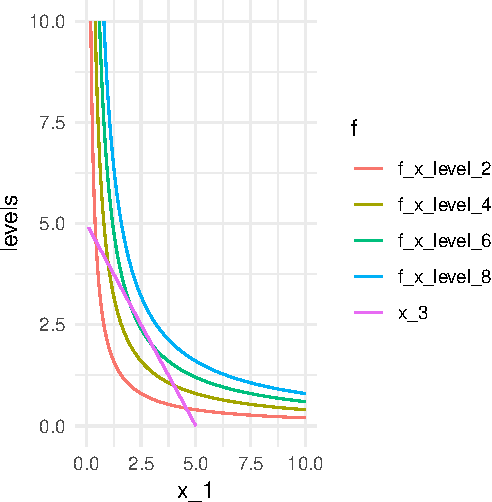
\includegraphics{Optimization_2_files/figure-latex/opt_dim_2_eq_constr-1} \end{center}

Geometrically we need to find the highest valued level set for
\(f(x) = x_1x_2\) that satisfies \(x_1+x_2=5, x_1, x_2\geq 0\). The key
observation is the following: at the optimal, the levels sets and the
constraint set must be tangent---just touching (intersecting) each other
at exactly one point. (Why must this be so? What happens if the plots
cross over? Can we improve the objective function then?)

\subsection{The Lagrangian}\label{the-lagrangian}

If the curves are tangents to each other at the optimal point then it
must be so that the tangents to the curves at the optimal are in the
same direction.

The slope of the level set of \(f\) at \(x^*\) is: \[
-\frac{\frac{\partial f}{\partial x_1}(x^*)}{\frac{\partial f}{\partial x_2}(x^*)}
\] and that of the equality constraint is: \[
-\frac{\frac{\partial h}{\partial x_1}(x^*)}{\frac{\partial h}{\partial x_2}(x^*)}
\] Since they're equal \[
\frac{\frac{\partial f}{\partial x_1}(x^*)}{\frac{\partial f}{\partial x_2}(x^*)} =
\frac{\frac{\partial h}{\partial x_1}(x^*)}{\frac{\partial h}{\partial x_2}(x^*)} =
\lambda
\] This can be rearranged as: \[
\frac{\frac{\partial f}{\partial x_1}(x^*)}{\frac{\partial h}{\partial x_1}(x^*)} =
\frac{\frac{\partial f}{\partial x_2}(x^*)}{\frac{\partial h}{\partial x_2}(x^*)} =
\lambda
\] or, \[
\frac{\partial f}{\partial x_1}(x^*)-\lambda\frac{\partial h}{\partial x_1}(x^*)=0
\] \[
\frac{\partial f}{\partial x_2}(x^*)-\lambda\frac{\partial h}{\partial x_2}(x^*)=0
\] There are three unknowns:\((x_1^*, x_2^*, \lambda)\). There are two
equations above, and there is a third equation---the constraint equation
\(h(x_1, x_2) = c_1\). Together, we can find \(x^*\) and \(\lambda\).

The following function is formally referred to as the \emph{Lagrangian},
and \(\lambda\) as the Lagrange multiplier: \[
\mathcal{L}(x_1,x_2,\lambda) := f(x_1,x_2)-\lambda\cdot(h(x_1,x_2)-c)
\]

We consider the critical points of the Lagrangian:
\(\frac{\partial \mathcal{L}}{\partial x_1}(x^*), \frac{\partial \mathcal{L}}{\partial x_2}(x^*), \frac{\partial \mathcal{L}}{\partial \lambda}(x^*)=0\).

Essentially by forming the Lagrangian, we are transforming a constrained
optimization program featuring the objective function \(f(\cdot)\) into
an \emph{unconstrained} optimization program featuring the Lagrangian
\(\mathcal{L}(\cdot)\). However, there is an extra variable \(\lambda\),
the Lagrange multiplier, that is introduced in the new program.

\subsubsection{Constraint Qualification}\label{constraint-qualification}

In order for the slopes to be well-defined,
\(\frac{\partial h}{\partial x_1}(x^*)\neq 0\) and
\(\frac{\partial h}{\partial x_2}(x^*)\neq 0\). Since this is a
restriction on the constraint set, it's called a \emph{constraint
qualification}.

\textbf{Theorem:} For the function
\(f:\mathbb{R}^n\to \mathbb{R}, f\in C^1\), if \(x^*\in \mathbb{R}^n\)
is a solution of \[\max f(x): x\geq 0, h(x)=c_1\] and \(x^*\) is
\emph{not} a critical point of \(h\); then, there is a real number
\(\lambda^*\) such that \((x^*,\lambda^*)\) is a critical point of
\(\mathcal{L}=f(x)-\lambda\cdot(h(x)-c)\).

\subsection{Level-Set Gradients and
Lagrangians}\label{level-set-gradients-and-lagrangians}

\begin{Shaded}
\begin{Highlighting}[]
\NormalTok{f_x_level_star <-}\StringTok{ }\FloatTok{6.4}\OperatorTok{/}\NormalTok{x_}\DecValTok{2} \CommentTok{#set manually}

\NormalTok{data_plot_grad <-}\StringTok{ }\KeywordTok{cbind}\NormalTok{(x_}\DecValTok{1}\NormalTok{, }
\NormalTok{                        f_x_level_star,}
\NormalTok{                        x_}\DecValTok{3}
\NormalTok{                        ) }\OperatorTok
\StringTok{  }\NormalTok{dplyr}\OperatorTok{::}\KeywordTok{as_tibble}\NormalTok{() }\OperatorTok
\StringTok{  }\NormalTok{tidyr}\OperatorTok{::}\KeywordTok{gather}\NormalTok{(.,}
                \KeywordTok{c}\NormalTok{(f_x_level_star, x_}\DecValTok{3}\NormalTok{),}
                \DataTypeTok{key =} \StringTok{'f'}\NormalTok{,}
                \DataTypeTok{value =} \StringTok{'levels'}
\NormalTok{                )}

\KeywordTok{ggplot}\NormalTok{(data_plot_grad, }\KeywordTok{aes}\NormalTok{(x_}\DecValTok{1}\NormalTok{, levels, }\DataTypeTok{color =}\NormalTok{ f)) }\OperatorTok{+}
\StringTok{  }\KeywordTok{geom_line}\NormalTok{() }\OperatorTok{+}
\StringTok{  }\KeywordTok{scale_y_continuous}\NormalTok{(}\DataTypeTok{limits =} \KeywordTok{c}\NormalTok{(}\DecValTok{0}\NormalTok{, }\DecValTok{10}\NormalTok{)) }\OperatorTok{+}
\StringTok{  }\KeywordTok{geom_segment}\NormalTok{(}\KeywordTok{aes}\NormalTok{(}\DataTypeTok{x =} \FloatTok{2.5}\NormalTok{,}
                   \DataTypeTok{y =} \FloatTok{2.5}\NormalTok{,}
                   \DataTypeTok{xend =} \FloatTok{3.75}\NormalTok{, }\CommentTok{#set manually}
                   \DataTypeTok{yend =} \DecValTok{3}
\NormalTok{                   ),}
               \DataTypeTok{color =} \StringTok{"blue"}\NormalTok{,}
               \DataTypeTok{arrow =} \KeywordTok{arrow}\NormalTok{(}\DataTypeTok{length =} \KeywordTok{unit}\NormalTok{(}\FloatTok{0.015}\NormalTok{, }\StringTok{"npc"}\NormalTok{)),}
               \DataTypeTok{size =} \FloatTok{0.2}
\NormalTok{               ) }\OperatorTok{+}
\StringTok{  }\KeywordTok{theme_minimal}\NormalTok{()}
\end{Highlighting}
\end{Shaded}

\begin{center}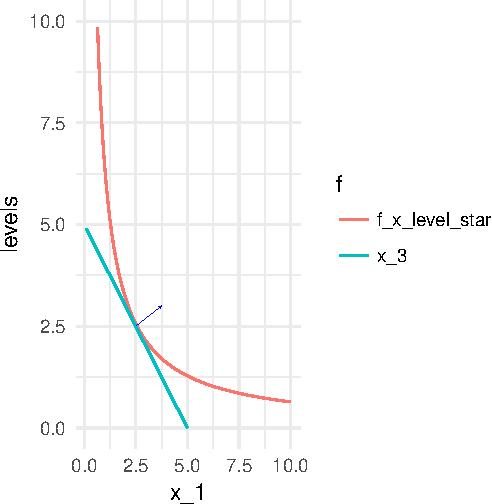
\includegraphics{Optimization_2_files/figure-latex/opt_dim_2_eq_grad-1} \end{center}

The gradient of \(f\) and \(h\) are respectively
\([\frac{\partial f}{\partial x_1}, \frac{\partial f}{\partial x_2}]\)
and
\([\frac{\partial h}{\partial x_1}, \frac{\partial f}{\partial x_2}]\).
These point to the directions of maximum change and are orthogonal to
the level sets of \(f, h\).

Since the level sets and the constraints are tangent at the optimal
implies that their respective gradients---orthogonal to the
tangent---must again point in the same direction.

\[
[\frac{\partial f}{\partial x_1}, \frac{\partial f}{\partial x_2}] = 
\lambda [\frac{\partial h}{\partial x_1}, \frac{\partial h}{\partial x_1}]
\]

This yields exactly the Lagrangian function for the optimization
program.

\subsection{Several Equality
Constraints}\label{several-equality-constraints}

Consider the following variation on the maximization problem where there
are several equality constraints now:

\[
\max f(x): x\in \mathbb{R}^n, x\geq 0
\] \[
C_h = \{h_1(x)=c_1,\hdots, h_m(x)=c_m\}
\]

The generalization from one to many equality constraints is
straightforward.

\subsubsection{Constraint
Qualification}\label{constraint-qualification-1}

In the case of one constraint, the qualification is:
\[[\frac{\partial h}{\partial x_1}(x^*),\hdots,\frac{\partial h}{\partial x_n}(x^*)]\neq (0,\hdots,0)\]

Likewise, in the case of \(m\) equality constraints:
\(\{h_1(x)=c_1,\hdots, h_m(x)=c_m\}\), their \emph{Jacobian} (first
derivative matrix) must be \emph{invertible} at the critical point
\(x^*\).

\[
Dh(x^*) = \begin{bmatrix}
\frac{\partial h_1}{\partial x_1}(x^*),\hdots,\frac{\partial h_1}{\partial x_n}(x^*)\\
\frac{\partial h_2}{\partial x_1}(x^*),\hdots,\frac{\partial h_2}{\partial x_n}(x^*)\\
 \vdots \\
\frac{\partial h_m}{\partial x_1}(x^*),\hdots, \frac{\partial h_m}{\partial x_n}(x^*)
\end{bmatrix}
\]

For the constraint Jacobian at the critical point required to be
invertible implies that the matrix above must have \emph{full rank},
further equivalent to the condition that the determinant be non-zero at
the critical point. More formally, it is said that \((h_1,\hdots,h_m)\)
satisfy the \emph{non-degenrate constraint qualification} (NCDQ) at
\(x^*\) if matrix \(Dh(x^*)\) is invertible at \(x^*\) (has full rank).

\subsubsection{The Geometry of the
Lagrangian}\label{the-geometry-of-the-lagrangian}

When there are \(m\) constraints: \(h_1(x)=c_1,\hdots,h_m(x)=c_m\), the
gradient of the objective function \(\nabla f(x^*)\) at the optimal must
be a linear combination of the gradients of the constraints
\(\sum_{i=1}^m \lambda_i \nabla h_i(x^*)\).

This is so because \(\nabla h_i\) gives the directions of maximum
increase of \(h_i\). If the constraints \(h_i=c_i\) are to be satisfied,
we must move in the direction where \(h_i\) are constant (and equal to
\(c_i\)) and hence in directions \emph{orthogonal} (perpendicular) to
\(\nabla h_i\) and hence in directions \emph{orthogonal} to
\(\sum_{i=1}^m \lambda_i \nabla h_i(x^*)\). In the same way, the contour
lines for \(f\) are orthogonal to \(\nabla f\).

At the optimal, the objective function \(f\) must touch (be tangent to)
the binding constraints and hence the gradient of \(f\) must lie in the
\emph{span} of the constraints' gradients:
\(\nabla f(x^*)=\sum_{i=1}^m \lambda_i \nabla h_i(x^*)\).

\textbf{Theorem:} Given
\(f, h_1, \hdots, h_m:\mathbb{R}^n\to \mathbb{R}\in C^1\), where \(f\)
is the objective function and \(h_i=c_i\) are equality constraints which
\(x\) must satisfy; and that \(h_i\) satisfiy the NDCQ condition; then
there are \(\lambda^*=(\lambda_1^*,\hdots,\lambda_m^*)\) such that
\((x^*,\lambda^*)\) is the critical point of the Lagrangian
\(\mathcal{L}(x,\lambda)\).

Hence \[
\mathcal{L}(x,\lambda) := f(x)-\lambda_1\cdot(h_1(x)-c_1)+\hdots+\lambda_m\cdot(h_m(x)-c_m)
\] and \[
\frac{\partial\mathcal{L}}{\partial x_1}(x^*,\lambda^*)=0,\hdots,\frac{\partial \mathcal{L}}{\partial x_n}(x^*,\lambda^*)=0
\] \[
\frac{\partial\mathcal{L}}{\partial \lambda_1}(x^*,\lambda^*)=0,\hdots,\frac{\partial \mathcal{L}}{\partial \lambda_m}(x^*,\lambda^*)=0
\] In total we get \(n+m\) equations with \(n+m\) unknowns:
\((x_1,\hdots,x_n,\lambda_1,\hdots,\lambda_m)\).

\section{Inequality Constraints}\label{inequality-constraints}

Consider now a maximization program in \(\mathbb{R}^2\) with one
inequality constraint: \[
\max f(x_1, x_2), (x_1, x_2)\geq 0, g(x_1, x_2)\leq b
\]

\subsection{Binding Constraint}\label{binding-constraint}

To make the discussion more concrete, reconsider the maximization of the
objective function \(f=x_1x_2\) with an inequality constraint
\(g(x) = x_1^2+x_2^2\leq 1\).

We can see that for such a maximization program, the optimal must occur
at the boundary of the constraint set \(g(x)=b\). The level sets of
\(f, g\) are tangent to each other, or equivalently their gradients are
in the same direction:

\[\nabla f(x^*) = \lambda \nabla g(x^*)\]

Additionally, however we note that \(\lambda > 0\) i.e., the gradients
point in the same direction and \emph{not} in the opposite direction as
is seen below.

\begin{Shaded}
\begin{Highlighting}[]
\NormalTok{x_}\DecValTok{4}\NormalTok{ <-}\StringTok{ }\KeywordTok{sqrt}\NormalTok{(}\DecValTok{1} \OperatorTok{-}\StringTok{ }\NormalTok{x_}\DecValTok{2}\OperatorTok{^}\DecValTok{2}\NormalTok{) }\CommentTok{#inequality constraint}

\NormalTok{f_x_level_}\DecValTok{1}\NormalTok{ <-}\StringTok{ }\DecValTok{1}\OperatorTok{/}\NormalTok{x_}\DecValTok{2}
\NormalTok{f_x_level_half <-}\StringTok{ }\DecValTok{1}\OperatorTok{/}\NormalTok{(}\DecValTok{2}\OperatorTok{*}\NormalTok{x_}\DecValTok{2}\NormalTok{)}
\NormalTok{f_x_level_qtr <-}\StringTok{ }\DecValTok{1}\OperatorTok{/}\NormalTok{(}\DecValTok{4}\OperatorTok{*}\NormalTok{x_}\DecValTok{2}\NormalTok{)}
\NormalTok{f_x_level_eighth <-}\StringTok{ }\DecValTok{1}\OperatorTok{/}\NormalTok{(}\DecValTok{8}\OperatorTok{*}\NormalTok{x_}\DecValTok{2}\NormalTok{)}

\NormalTok{data_plot_ineq <-}\StringTok{ }\KeywordTok{cbind}\NormalTok{(x_}\DecValTok{1}\NormalTok{, }
\NormalTok{                        f_x_level_half,}
\NormalTok{                        f_x_level_}\DecValTok{1}\NormalTok{,}
\NormalTok{                        f_x_level_}\DecValTok{2}\NormalTok{,}
\NormalTok{                        f_x_level_eighth,}
\NormalTok{                        f_x_level_qtr,}
\NormalTok{                        x_}\DecValTok{4}
\NormalTok{                        ) }\OperatorTok
\StringTok{  }\NormalTok{dplyr}\OperatorTok{::}\KeywordTok{as_tibble}\NormalTok{() }\OperatorTok
\StringTok{  }\NormalTok{tidyr}\OperatorTok{::}\KeywordTok{gather}\NormalTok{(.,}
\NormalTok{                f_x_level_half}\OperatorTok{:}\NormalTok{x_}\DecValTok{4}\NormalTok{,}
                \DataTypeTok{key =} \StringTok{'f'}\NormalTok{,}
                \DataTypeTok{value =} \StringTok{'levels'}
\NormalTok{                )}

\KeywordTok{ggplot}\NormalTok{(data_plot_ineq, }\KeywordTok{aes}\NormalTok{(x_}\DecValTok{1}\NormalTok{, levels, }\DataTypeTok{color =}\NormalTok{ f)) }\OperatorTok{+}
\StringTok{  }\KeywordTok{geom_line}\NormalTok{() }\OperatorTok{+}
\StringTok{  }\KeywordTok{scale_y_continuous}\NormalTok{(}\DataTypeTok{limits =} \KeywordTok{c}\NormalTok{(}\DecValTok{0}\NormalTok{, }\DecValTok{2}\NormalTok{)) }\OperatorTok{+}
\StringTok{  }\KeywordTok{scale_x_continuous}\NormalTok{(}\DataTypeTok{limits =} \KeywordTok{c}\NormalTok{(}\DecValTok{0}\NormalTok{, }\DecValTok{3}\NormalTok{)) }\OperatorTok{+}
\StringTok{  }\KeywordTok{theme_minimal}\NormalTok{()}
\end{Highlighting}
\end{Shaded}

\begin{center}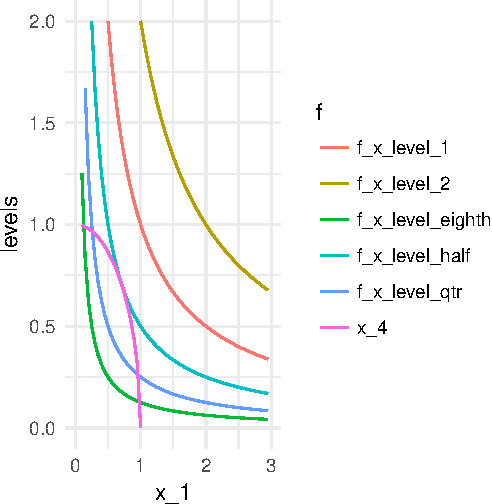
\includegraphics{Optimization_2_files/figure-latex/opt_dim_2_ineq-1} \end{center}

As before, the constraint qualification condition holds---the optimal
should not be a critical point of the inequality constraint.

\subsection{Non-binding Constraint}\label{non-binding-constraint}

When constraints are of the form \(g(x)\leq b\), the optimal may as well
lie strictly in the interior depending upon the objective function
contour lines. In such cases, we can still form the Lagrangian provided
we enforce the condition that \(\lambda=0\), which when combined with
the slackness of the inequality: \(g(x)-b<0\) gives complementary
slackness conditions: \(\lambda\cdot (g(x)-b)=0\).

Since we do not know which constraint is non-binding at the optimal, we
cannot set \(\frac{\partial \mathcal{L}}{\partial \lambda}=0\) (which is
equivalent to \(g(x)-b=0\)). Hence such a condition is replaced by the
complementary slackness condition, which implies that either the
constraint is binding, in which case \(\lambda>0\) or the constraint is
slack in which case \(\lambda = 0\).

\textbf{Theorem:} Given functions
\(f,g:\mathbb{R}^2\to \mathbb{R}\in C^1\) and that \(g(x_1, x_2)\leq b\)
(additionally, if \(g(x^*)=b\), then \(\nabla g(x^*)\neq 0\)); then
\((x^*,\lambda^*)\) is the critical point of the Lagrangian and the
following are true:

\begin{enumerate}
\def\labelenumi{\arabic{enumi}.}
\tightlist
\item
  \(\nabla_{x^*,\lambda^*} \mathcal{L}=0\)
\item
  \(\lambda^*\cdot(g(x^*)-b)=0\)
\item
  \(\lambda^*\geq 0\)
\end{enumerate}

\subsubsection{Remarks}\label{remarks}

\begin{enumerate}
\def\labelenumi{\arabic{enumi}.}
\tightlist
\item
  \(\nabla_{x}\mathcal{L}=0\) for both equality and inequality
  constraints.
\item
  \(\nabla_{\lambda}\mathcal{L}=0\) is true \emph{only} for equality
  constraints.
\item
  Constraint qualification needs to be checked \emph{only} for binding
  inequality constraints.
\item
  \(\lambda\geq 0\) \emph{only} for inequality constraints.
\item
  Complementary slackness must hold for inequality constraints.
\end{enumerate}

\subsection{Several Inequality
Constraints}\label{several-inequality-constraints}

The generalization from one inequality constraint to several is fairly
straightforward:

\textbf{Theorem:} Given functions
\(f, g_1,\hdots,g_k:\mathbb{R}^n\to \mathbb{R}\in C^1\) and
\(x^*\in \mathbb{R}^n\) is a local maximizer on the constraint set

\[C_g=\{g_1(x)\leq b_1,\hdots,g_k(x)\leq b_k\}\]

Assume without loss of generality that the first \(k_0\) constraints are
binding at \(x^*\) and the rest \(k-k_0\) are slack. Also assume the
nondegeneracy constraint qualification is satisfied by stipulating that
the following constraint derivative matrix is invertible at the optimal
\(x^*\)

\[
Dg(x^*) = \begin{bmatrix}
\frac{\partial g_1}{\partial x_1}(x^*), \hdots, \frac{\partial g_1}{\partial x_n}(x^*)\\
\vdots\\
\frac{\partial g_{k_0}}{\partial x_1}(x^*), \hdots, \frac{\partial g_{k_0}}{\partial x_n}(x^*)
\end{bmatrix}
\]

That is, the constraint Jacobian at the critical point is invertible and
has full rank.

Then the Lagrangian
\[\mathcal{L}(x,\lambda):=f(x)-\lambda_1\cdot(g_1(x)-b_1)-\hdots-\lambda_k(g_k(x)-b_k)\]
has the critical points \((x^*,\lambda^*)\) such that:

\begin{enumerate}
\def\labelenumi{\arabic{enumi}.}
\tightlist
\item
  \(\nabla_x\mathcal{L}(x^*)=0\)
\item
  \(\lambda_1^*\cdot(g_1(x)-b_1)=0,\hdots,\lambda_k^*\cdot(g_k(x)-b_k)=0\)
\item
  \(\lambda_1^*\geq 0,\hdots, \lambda_k^*\geq 0\)
\end{enumerate}

\section{The General Case: Mixed
Constraints}\label{the-general-case-mixed-constraints}

The Karush-Kuhn-Tucker (KKT) conditions are first order necessary
conditions for a general optimization program including equality as well
as inequality constraints. If there are no inequality constraints, the
KKT conditions are equivalent to the method of Lagrange multipliers.

We consider the general case: \[\max f(x), x\in \mathbb{R}^n, x\geq 0:\]
\[C_g=\{g_1(x)\leq b_1,\hdots,g_k(x)\leq b_k\}\]
\[C_h=\{h_1(x)=c_1,\hdots,h_m(x)=c_m\}\]

We assume
\(f,\{g_i\}_{i=1}^k,\{h_j\}_{j=1}^m:\mathbb{R}^n\to \mathbb{R}\in C^1\).

For the inequality constraint set \(C_g\), we assume without loss of
generality that the first \(k_0\) constraints are binding at \(x^*\). We
assume that the following derivative matrix is invertible at the optimal
(NDCQ) (has full rank):

\[
\begin{bmatrix}
\frac{\partial g_1}{\partial x_1}(x^*),\hdots,\frac{\partial g_{1}}{\partial x_n}(x^*)\\
\vdots\\
\frac{\partial g_{k_0}}{\partial x_1}(x^*),\hdots,\frac{\partial g_{k_0}}{\partial x_n}(x^*)\\
\vdots\\
\frac{\partial h_1}{\partial x_1}(x^*),\hdots,\frac{\partial h_1}{\partial x_n}(x^*)\\
\vdots\\
\frac{\partial h_m}{\partial x_1}(x^*),\hdots,\frac{\partial h_m}{\partial x_n}(x^*)
\end{bmatrix}
\]

We form the Lagrangian as before:

\[
\mathcal{L}(x,\lambda,\mu) := f(x)-\sum_{i=1}^k \lambda_i\cdot(g_i(x)-b_i)-
\sum_{j=1}^m \mu_j\cdot(h_i(x)-c_i)
\]

The critical points of the Lagrangian are found from the FOC: \[
\nabla_x\mathcal{L}(x^*,\lambda^*,\mu^*) := \nabla f(x^*)-
\sum_{i=1}^k\lambda_i\nabla g_i(x^*) -
\sum_{j=1}^m\mu_j\nabla h_j(x^*)=0
\]

The Lagrangian above has multipliers
\(\lambda^*\in \mathbb{R}^k, \mu^*\in \mathbb{R}^m\) such that

\begin{enumerate}
\def\labelenumi{\arabic{enumi}.}
\tightlist
\item
  \(\nabla_x\mathcal{L}(x^*,\lambda^*)=0\)
\item
  \(\lambda_1\cdot(g_1(x^*)-b_1)=0,\hdots,\lambda_k\cdot(g_k(x^*)-b_k)=0\)
\item
  \(h_1(x^*)-c_1=0,\hdots,h_m(x^*)-c_m=0\)
\item
  \(\lambda_1^*\geq 0,\hdots,\lambda_k^*\geq 0\)
\item
  \(g_1(x^*)-b_1\leq 0,\hdots,g_k(x^*)-b_k\leq 0\)
\end{enumerate}

\section{Interpreting the Lagrange
Multiplier}\label{interpreting-the-lagrange-multiplier}

In plain language, the Lagrange multiplier measures the sensitivity of
the optimal value of the objective function to changes in the
constraints' right hand sides.

We illustrate this idea using a simple maximization program in two
dimensions and with one equality constraint:

\[\max f(x),x\in \mathbb{R}^2,x\geq 0:\] \[h(x)=c\]

The central idea is to consider \(c\) as a parameter that varies from
problem to problem. Given \(c\), \((x_1^*(c),x_2^*(c))\) is the optimal
as a function of the constraint parameter \(c\);
\(f(x_1^*(c),x_2^*(c))\) is the optimal value as a function of
constraint parameter; and \(\lambda^*(c)\) is the corresponding
multiplier.

\textbf{Theorem:} Given \(f,h:\mathbb{R}^2\to \mathbb{R}\in C^1\); given
\(x_1^*(c),x_2^*(c),\lambda^*(c)\in C^1\) and NDCQ condition:
\[\lambda^*(c)=\frac{d}{dc}\cdot [f(x_1^*(c),x_2^*(c))]\]

The same idea can be generalized for the case with several mixed
constraints.

\section{Application: Portfolio
Optimization}\label{application-portfolio-optimization}

The original mean-variance framework admits a quadratic program that may
be solved via \texttt{quadprog()}. However, as has been argued
effectively, variance is but a poor measure of risk. As opposed to
variance, which penalizes both positive and negative deviations from the
mean equally, a true risk measure should penalize only negative
deviations since risk emanates from losses but \emph{not} from gains.

Hence a general portfolio optimization program where risk is measured
via some function \(\rho(\cdot)\) is \[\min{} \rho(w):\] \[w^{\top}e=1\]
\[w^{\top}\mu \geq \mu_*\] \[w\geq 0\]

Some common measures of portfolio risk are ``variance'',
``Value-at-Risk'' (VaR); ``Average Value-at-Risk'' (AVaR); and many
others. For the case when the risk measure is variance, the resulting
optimization framework is the mean-variance framework.

\subsection{Constraints}\label{constraints}

Depending upon institutional frameworks, there are many extra
constraints that a portfolio manager may need to satisfy. We discuss
some prominent ones below that are either linear or quadratic in nature.

\subsubsection{Long-only Constraint}\label{long-only-constraint}

We've been imposing this constraint implicitly whenever we've insisted
on the constraint \(w\geq 0\). \(w_j<0\) implies that for security \(j\)
one has negative weight---implying the use of borrowed money for use of
asset \(j\).

\subsubsection{Holding Constraints}\label{holding-constraints}

For constraints that stipulate that the securitiy weights be between
maximal and minimal limits: \[L_i\leq w_i \leq U_i\]

\subsubsection{Turnover Constraints}\label{turnover-constraints}

High turnovers may lead to high transaction costs. There could be
mandates for turnover constraints on individual securities as well as on
the entire portfolio. If the current weights are \(w_0\) and targeted
weights are \(w\) then the turnover constraint for security \(i\)
manifests as: \[|w-w_0|_i\leq U_i\]

And for the whole portfolio: \(\sum_{i=1}^n |w-w_0|_i\leq U_{port}\)

\subsubsection{Tracking Error
Constraints}\label{tracking-error-constraints}

A very coarse classification of fund management is between ``active''
and ``passive'' funds. Active managers assume that there are pockets of
inefficiency in financial markets and try to exploit them to beat the
market. Passive fund managers assume that markets are more or less
efficient and aim to mimic the market index as a whole. Today passive
indexing is an extremely popular type of fund management.

Often managers of passive and/or index funds are tasked with
\emph{following} an index, say the S\&P500. The idea is that the fund
manager replicates the index performance---if the index posts high
gains, the investors in the fund reap benefits; and if the index does
poorly, so do the investors.

If \(w_b\) are the benchmark market capitalization weights for an index
and \(r\) the return vector, the benchmark returns are
\(w_b^{\top}r = r_b\). A passive fund manager may choose to impose the
following restriction on portfolio weights:

\[\|w-w_b\|\leq M\]

The most common metric to be used for this purpose is the ``tracking
error'' which is the variance of the difference between the portfolio
and benchmark returns.

\[\text{TE}_p = \text{var}(r_p-r_b)=\text{var}(w^{\top}r-w^{\top}_b r)\]
\[\text{TE}_p = (w-w_b)^{\top}\text{var}(r)(w-w_b)=(w-w_b)^{\top}\Sigma(w-w_b)\]

To insist that the tracking error be less than a critical value
introduces the following constraint:
\[(w-w_b)^{\top}\Sigma(w-w_b)\leq \sigma^2_{TE}\]

Hence the benchmark tracking problem can be framed as:

\[\min_w{} (w-w_b)^{\top}\Sigma(w-w_b):\] \[w^{\top}e = 1 \]

\subsection{Computation: Portfolio
Optimization}\label{computation-portfolio-optimization}

Let's revisit the mean-variance problem from before.

There are two normally distributed common stocks whose expected returns
are \(\mu^{\top} = (1.8\%, 2.5\%)\) with covariance matrix \(\Sigma\):

\[\Sigma = 
\begin{bmatrix}
1.68, 0.34\\
0.34, 3.09\\
\end{bmatrix}
\]

The minimization program was:

\[\min{} 1.68w_1^2+3.09w_2^2+2*0.34w_1w_2:\] \[w_1+w_2=1\]
\[0.018w_1 + 0.025w_2 \geq 0.018\] \[w_1, w_2\geq 0\]

However, in the new problem suppose there is a holding constraint: the
manager cannot have any stock weigh more than 60\%.\footnote{This
  constraint could be needed to avoid over-reliance on one stock lest it
  perform poorly sometime and take the portfolio down with it. Note that
  the previous problem where this constraint does not feature suggests
  best weight for the first stock to be 0.67, which will be infeasible
  in this case.}

Hence the new minimization program becomes:

\[\min{} 1.68w_1^2+3.09w_2^2+2*0.34w_1w_2:\] \[w_1+w_2=1\]
\[0.018w_1 + 0.025w_2 \geq 0.018\] \[w_1\leq 0.60\] \[w_2\leq 0.60\]
\[w_1, w_2\geq 0\]

We can solve this via \texttt{quadprog} using the \texttt{solve.QP()}
function.

\begin{Shaded}
\begin{Highlighting}[]
\NormalTok{D_mat <-}\StringTok{ }\DecValTok{2}\OperatorTok{*}\KeywordTok{matrix}\NormalTok{(}\KeywordTok{c}\NormalTok{(}\FloatTok{1.68}\NormalTok{, }\FloatTok{0.34}\NormalTok{, }\FloatTok{0.34}\NormalTok{, }\FloatTok{3.09}\NormalTok{), }\DecValTok{2}\NormalTok{, }\DecValTok{2}\NormalTok{) }\CommentTok{#why 2*?}
\NormalTok{d_vec <-}\StringTok{ }\KeywordTok{matrix}\NormalTok{(}\DecValTok{0}\NormalTok{, }\DecValTok{0}\NormalTok{, }\DataTypeTok{nrow =} \DecValTok{2}\NormalTok{, }\DataTypeTok{ncol =} \DecValTok{1}\NormalTok{)}
\NormalTok{A_mat <-}\StringTok{ }\KeywordTok{matrix}\NormalTok{(}\KeywordTok{c}\NormalTok{(}\DecValTok{1}\NormalTok{, }\DecValTok{1}\NormalTok{, }\FloatTok{0.018}\NormalTok{, }\FloatTok{0.025}\NormalTok{, }\OperatorTok{-}\DecValTok{1}\NormalTok{, }\DecValTok{0}\NormalTok{, }\DecValTok{0}\NormalTok{, }\OperatorTok{-}\DecValTok{1}\NormalTok{), }
                \DataTypeTok{nrow =} \DecValTok{4}\NormalTok{, }
                \DataTypeTok{byrow =}\NormalTok{ T}
\NormalTok{                )}
\NormalTok{b_vec <-}\StringTok{ }\KeywordTok{c}\NormalTok{(}\DecValTok{1}\NormalTok{, }\FloatTok{0.018}\NormalTok{, }\OperatorTok{-}\FloatTok{0.60}\NormalTok{, }\OperatorTok{-}\FloatTok{0.60}\NormalTok{)}
\NormalTok{m_eq <-}\StringTok{ }\DecValTok{1}

\NormalTok{quadprog}\OperatorTok{::}\KeywordTok{solve.QP}\NormalTok{(D_mat, d_vec, }\KeywordTok{t}\NormalTok{(A_mat), b_vec, m_eq) }\CommentTok{#note t(A_mat)}
\end{Highlighting}
\end{Shaded}

\begin{verbatim}
## $solution
## [1] 0.6 0.4
## 
## $value
## [1] 1.2624
## 
## $unconstrained.solution
## [1] 0 0
## 
## $iterations
## [1] 3 0
## 
## $Lagrangian
## [1] 2.880 0.000 0.592 0.000
## 
## $iact
## [1] 1 3
\end{verbatim}


\end{document}
